\documentclass[11pt]{extarticle}
\usepackage[spanish,english]{babel}
\usepackage[utf8]{inputenc}
\usepackage[letterpaper,margin=2.54cm]{geometry}
\usepackage{graphicx}
\usepackage[spanish]{babel}
\usepackage{titlesec}
\usepackage{tocloft}%
\graphicspath{/Users/mijatola/Documents/Tesis}
\selectlanguage{spanish}
\let \savenumberline \numberline
\def \numberline#1{\savenumberline{#1.}}

\date{}
\author{}

\begin{document}

\title{
    \textbf{
      \Large{UNIVERSIDAD MAYOR DE SAN ANDR\'ES}\\
      \normalsize{
        FACULTAD DE CIENCIAS PURAS Y NATURALES\\
        CARRERA DE INFORM\'ATICA\\
      }
      \hfill \break
      
\includegraphics[width=5cm,height=11cm]{umsa}
      \break
      \begin{large}
        PERFIL DE TESIS DE GRADO
        \break
        \break
        MODELO GENERADOR DE GRAFOS ALEATORIOS 
      \end{large}
      \break
      \break
      \small{
        Para obtener el Título de Licenciatura en Informática \break
        Mención Ingeniería de Sistemas Informáticos\break
      }
      \break
      \large {
        POR: CARLOS MIJAEL TOLA APAZA\\
        TUTOR: LIC. JORGE TERAN
      }
      \break
      \small {
        LA PAZ - BOLIVIA \break
        Noviembre, 2021
      }
    }
}

\maketitle
\selectlanguage{spanish}
\tableofcontents
\newpage

\titleformat*{\section}{\normalsize\bfseries\MakeUppercase}
\titleformat*{\subsection}{\normalsize\bfseries\MakeUppercase}
\titlelabel{\thetitle.\quad}

\newcommand\justificacion{Justificaci\'on }
\newcommand\guion{\item[-]}

\renewcommand{\labelenumii}{\arabic{enumi}.\arabic{enumii}}
\renewcommand{\labelenumiii}{\arabic{enumi}.\arabic{enumii}.\arabic{enumiii}}
\renewcommand{\labelenumiv}{\arabic{enumi}.\arabic{enumii}.\arabic{enumiii}.\arabic{enumiv}}

\section{Introduccion} 
Una red o grafo es un sistema compuesto por objetos discretos (v\'ertices) y una relación (arista) entre algunos pares
de ellos. Son herramientas de modelado ubicuas en muchos campos de investigación. 
Algunos ejemplos comunes incluyen redes sociales, neuronales, de proteínas y de comunicación.
Hoy en dia con el poder de computo disponible, han hecho que el estudio de redes y
herramientas para analizarlas sean temas en alza dentro de la comunidad académica.\hfill \break

Los grafos aleatorios son construcciones probabilísticas que permiten definir realizaciones
aleatorias de grafos. 
El uso generalizado de grafos aleatorios se ha destacado en el contexto de las  
aplicaciones de bases de datos y análisis de algoritmos durante 
varios años. Esto se debe a que tales estructuras de datos resultan ser muy útiles 
en muchas  aplicaciones, desde el análisis de redes complejas hasta el estudio de 
algoritmos aleatorios. Generar estos grafos de manera aleatoria tiene un nivel de dificultad
bastante alta, ya que al momento de generar un grafo se tienen que controlar algunas propiedades 
dependiendo el tipo de grafo que deseamos generar, por ejemplo: si el objetivo es construir un Arbol 
(Grafo conexo con \(E\) vertices y \(E - 1\) aristas)
se debe tener control sobre donde se genera un nuevo nodo y arista, verificando que no existan
ciclos, caso contrario el modelado no cumpliria con su objetivo. Tambien podriamos mencionar que construir
un Grafo Completo (Grafo con \(E\) vertices y \( \frac{E * (E - 1)}{2}\) aristas) tiene una complejidad No Polinomial NP, 
haciendo que sea solo posible generar grafos completos con un limite de 20 nodos aproximandamente.
Otro factor importante es que al ser este un modelado de grafos aleatorios, cada vertices a ser agregado,
tiene cierta probabilidad de ser tomado en cuenta en el grafo generado o no. \hfill\break 

Existen varios algoritmos generadores de grafos, como ser los modelos de grafos de Erdős-Rényi,
y algunas variantes de dicho modelado, que no generan grafos representativos (no se asemejan a redes del mundo real), no pueden generar grafos con grandes 
cantidades de vertices y se toman bastante tiempo en 
el generado [B2]. 
Dados estos argumentos,  el objetivo de este trabajo es crear un modelo generador de grafos aleatorios que sean representativos de 
forma eficiente. Cuando decimos representativos, nos referimos a Redes que se asemejen al mundo real y cuando decimos eficiente, nos referimos a: mejores tiempos de ejecucion para
el generado y el minimo uso de CPU, GPU y memoria comparando a modelos ya existentes. \hfill \break \break
Debido a que en Teoría de Grafos existe una infinidad de tipos de grafos, nos enfocaremos simplemente en un conjunto 
de grafos que son: Grafos directos acíclicos (DAG), Grafos Bipartitos, Grafos completos, 
Grafos no dirigidos conexos y no conexos, y árboles.

\section{Antecedentes}
El primer modelo de grafos aleatorios fue introducidos por P. Erdös en 1959 como una
herramienta para aplicar el método probabilístico para probar una relación asintótica entre
la cintura y el número cromático de grafos generales. Más tarde, junto con A. Rényi,
continuó el estudio de este modelo. Este es uno de los dos modelos conocidos
hoy en día como modelos de Erdös-Rényi. Consiste en la construcción de grafos finitos con un
número fijo de aristas distribuidas uniformemente a lo largo del conjunto de pares de vértices;
mientras que el segundo modelo que comparte el mismo nombre, se debe a E. Gilbert, y
consiste en grafos finitos obtenidos al establecer, independientemente y con la misma probabilidad, una arista entre cada par de vértices. A partir de ahí, se desarrollaron muchos modelos
de grafos aleatorios diferentes. Estos probaron ser no sólo construcciones interesantes, sino
también muy útiles en aplicaciones: como herramientas para estudiar escenarios promedio en
redes complejas y como una forma de explorar posibles mecanismos que dan lugar a muchas
de las características distintivas de las redes observadas en el mundo real. Por ejemplo, incluso
un modelo tan simple como el de Erdös-Rényi exhibe la propiedad del mundo pequeño (prevalencia de distancias relativamente cortas entre la mayoría de los pares de vértices) observada
en muchas redes sociales y de comunicación.

Al respecto de las investigaciones relacionadas con el tema podemos destacar las siguientes:

\begin{itemize}
  \item \textbf{Titulo:} Desempeño asintótico de algoritmos secuenciales
  en grafos aleatorios - Tesis presentada para optar al título de Doctor.\\
  \textbf{Autor:} Lic. Manuel Sáenz \\
  \textbf{A\~no:} 2019\\
  \textbf{Institucion:} Universidad de Buenos Aires\\
  En el mencionado trabajo, se estudia la evolucion y convergencia de algoritmos
  generadores de grafos, asi de esa forma lograr delimitar el algoritmo de modelado 
  de grafos Erdös-Rényi. Para demostrar sus limitaciones se demuestra que para los grafos
  generados por el modelo Erdös-Rényi es posible construir un conjunto independiente  maximo
  en tiempo polinomal. Pese a que el problema de construir Conjuntos Independientes Maximos es
  del tipo NP-dificil.

\end{itemize}

\begin{itemize}
  \item \textbf{Titulo:} Generación rápida de gráficos aleatorios\\
  \textbf{Autor:} Sadegh Heyrani, Nobari Xuesong Lu \\
  \textbf{A\~no:} 2011\\
  \textbf{Institucion:} Universidad Nacional de Singapore\\
  En el mencionado trabajo, se plante un modelo generador de grafos, usando programacion
  paralela y gpu junto a su algoritmo ER y ZER (creado por ellos). Los grafos que pueden ser
  generados por este modelado son: Grafos dirigidos y no dirigidos.
\end{itemize}

\begin{itemize}
  \item \textbf{Titulo:} Implementacion de un generador de topologias aleatorias en emulador de red mininet.\\
  \textbf{Autor:} Rosa Alejandra García Grisales, Juan Carlos Agudelo Calderón\\
  \textbf{A\~no:} 2015\\
  \textbf{Institucion:} Universidad Católica De Pereira\\
  En el mencionado trabajo, se plante implementar un generador de grafos para el emulador Mininet, que es 
  una aplicacion desarrollada para la investigacion de prototipos SDN en tiempo real.
  Este m\'etodo usa un Modelo de Waxmax (variante de Erdös-Rényi), que construye grafos en tiempo lineal, 
  pero usando bastante memoria limitando el generado a aproximandamente 1000 nodos solamente.
\end{itemize}

\begin{itemize}
  \item \textbf{Titulo:} Modelado de grafos aleatorios: una revisión de los conceptos\\
  \textbf{Autor:} Mikhail Drobyshevskiy, Denis Turdakov\\
  \textbf{A\~no:} 2019\\
  \textbf{Institucion:} Instituto de Física y Tecnología de Moscú\\
  En este trabajo, se hace una analisis a profundidad de el Algoritmo Erdös-Rényi.
  Se indentifico seis direcciones donde este modelos tienen sus aplicaciones: comprensión de redes, análisis, extrapolación, puntos de referencia, modelos nulos y aleatorización. 

\end{itemize}



\section{Planteamiento del problema}
  El modelado de grafos juega un rol importante en el an\'alisis de redes complejas. 
  Nos ayudan a entender, controlar predecir fen\'omenos que pueden ocurrir en redes sociales, 
  redes biol\'ogicas, internet y muchos mas. Aunque ya existen, varios modelos generadores de grafos, tales como el Modelado  Erdös-Rényi, esto no suelen ser representativos
  y al mismo tiempo son costosos en tiempo y memoria [B2].\hfill\break

  Otros autores han afirmado que:\\

  \footnotesize{
    En la era del BIG DATA, hay muchas redes masivas que deben explotarse y analizarse. Ya que
    tales redes no se pueden manejar en la memoria de una sola computadora, nuevos métodos de agrupamiento
    se han introducido para modelos avanzados de computación (Buzun et al., 2014; Zeng & Yu, 2016).
    Estos algoritmos utilizan representaciones de entrada jerárquicas, lo que implica que los experimentos realizados en Grafos de referencia de tamaño pequeño o mediano no se pueden utilizar para predecir el rendimiento en instancias mucho más grandes (Emmons et al., 2016). Desafortunadamente, muchos puntos de referencia de agrupamiento de gráficos
    Los generadores actualmente disponibles no pueden generar los Grafos del tamaño necesario (Bae & Howe,
    2015; Buzun et al., 2014).
  \textit{ (Artificial Benchmark for Community Detection (ABCD)—Fast random graph model with community structure, 2021)}
  }

  \subsection{Problema central}
     ¿Con que grado de fiabilidad los modelos generadores de grafos aleatorios Erdös-Rényi pueden construir grafos representativos en tiempo y coste de memoria minimos? 

\section{Hip\'otesis}
  El modelo para la generacion de grafos aleatorios usando GPU (Unidad de procesamiento gr\'afico) y programaci\'on paralela 
  representa estos Grafos en tiempo y memoria eficiente con una fiabilidad del 90\%.

  \subsection{Operacionalizaci\'on de variables}
  Se pudieron identificar las siguientes variables:\hfill \break \break
  \begin{tabular}{||c c c c||}
    \hline
    Concepto & Dimension & Indicador & Escala de medicion\\
    \hline
    Eficiencia &  & Tiempo de ejecucion & Segundos\\
              &   & Memoria usada en el proceso del generado & Megabytes\\
    \hline
    Representacion eficaz & & Grado  &  Numero Entero\\ 
              &   & Numero de componentes & Numero Entero\\
    \hline
    Aleatoriedad & & Entropia  & Numero Real\\
    \hline
  \end{tabular}

\section{Definicion de objectivos}
  \subsection{Objetivo general}
  Desarrolar un modelo generador de grafos aleatorios representativos y eficiente en tiempo y memoria.
  \subsection{Objetivos secundarios}
      \begin{itemize}
        \guion Analizar y diseñar un modelo generador de grafos aleatorios para: Grafos directos acíclicos (DAG), Grafos Bipartitos, Grafos completos, Grafos no dirigidos conexos y no conexos, y árboles.
        \guion Implementar el modelo generador de grafos.
        \guion Verificar que los tiempos al generar los grafos sean eficientes experimentalmente.
        \guion Verificar que el generador de grafos sea eficiente según su complejidad algorítmica.
      \end{itemize}
\section{\justificacion}
  \subsection{\justificacion econ\'omica}
    Para el analisis de diferentes redes, se requiere tener acceso a distintas redes de prueba, para su simulacion y estudio.
    Generar  estas redes o grafos de manera eficiente significa que se reduciran los costos de energia y se
    eliminara el tiempo invertido en dicho modelado.
  \subsection{\justificacion social}
    El impacto que tienen las redes sociales hoy en d\'ia en la sociedad ha marcado un hito en la forma de comunicarnos,
    debido a su creciemiento actual estas redes sociales siempre esta a la mejora de sus algorimos.
    Para esto es necesario investigar y probar dichos algoritmos en grafos aleatorias.
  \subsection{\justificacion cient\'fica}
    El presente trabajo combinara tecnicas algor\'itmicas, mascaras de bits, con tecnicas
    matematicas, Hashing, de tal manera que el modelado de las redes o grafos sea eficiente,
    esto se puede verificar usando notaciones de complejidad algor\'itmicas.
\section{Alcances y limites}
  \subsection{Alcances}
    \begin{itemize}
      \guion El presente trabajo diseñara un modelo generador de grafos aleatorios
            para DAGs, Grafos bipartitos, Grafos completos, Grafos no dirigidos
            conexos y no conexos, y arboles de manera eficiente.
      \end{itemize}
  \subsection{L\'imites}
    \begin{itemize}
      \guion Algunos tipos de grafos con construcciones y solucion no polinomial NP no seran tomados en cuenta.
    \end{itemize}

\section{Metodolog\'ia}
  Para el desarrollo del presente trabajo se utilizara un 
  \textbf{M\'etodo de investigacion experimental} para cumplir con los 
    objectivos propuestos para el modelo generador de grafos aleatorios. 
    Esta se dividirar en las siguientes etapas.
    \begin{enumerate}
      \item Recopilacion de informacion.
      \item Elaboracion del Modelo generador de grafos aleatorios.
      \item Pruebas de funcionamiento y/o presentación de mejoras para el modelo.
      \item Comparaciones y analisis de los datos.
      \item Conclusiones.
    \end{enumerate}
    
    La primera etapa se recopilara la informacion necesaria y
    se estudiara temas relacionadas al mismo.\hfill\break

    La segunda etapa se realizara el Modelo generado de grafos tomando
    encuenta los alcances y limites. \hfill\break

    La tercera etapa se verificara la funcionalidad del modelo.
    \hfill\break

    En la cuarta etapa se analizaran los datos y se los comparara con 
    otros modelos.
    \hfill\break

    En la ultima etapa, se presentaran los resultados finales, las
    conclusienes y recomendaciones con respecto al proyecto

    \begin{center}
      \begin{tabular}{||c | c||} 
       \hline
       ETAPAS & ACTIVIDADES\\ [0.5ex] 
       \hline\hline
       Recopilacion de informacion &  - Investigar la existenciaa de \\ & modelos generadores de grafos.\\
        & - Estudiar el proceso de generado\\ & de dichos modelos investigados.\\
       \hline
       Elaboracion del modelo & - Analizar y diseñar las \\ & etapas que necesitaran los modelados.\\
        & - Modelar el proceso generico, para construir\\
        & los grafos de forma aleatoria (Dirigidos y no Dirigidos). \\
        & - Modelaro el proceso para los distintos grafos\\ 
        & descritos en los alcances (DAG, Completos y Arboles).\\
       \hline
       Pruebas de funcionamiento y mejoras.
        & - Verificar el funcionamiento pleno del modelo.\\
        & - Aplicar las mejoras encontradas y propuestas.\\
       \hline
       Comparacion y Analisis & - Comparar el modelado propuesto \\
        & con respector al modelos ya existentes. \\
        & - Analizar de formar estadisticaa los datos devuelto\\
        &  de las comparaciones.\\
        & - Generalizar y encontrar la complejidad Algoritmica.\\
       \hline
       Conclusiones & - Presentar las conclusions\\ & obtenias al finalizar el trabajo. \\ 
       & - Compartir algunas recomendaciones \\ & obtenidas del trabajo realizado.\\
       \hline
      \end{tabular}
    \end{center}

\section{Bibliograf\'ia}
  [B1] Manuel Zaens. (2019). Desempeño asintotico de algoritmos secuenciales en grafos aleatorios. 2019, de Universidad de Buenos Aires Sitio web:\hfill\break http://cms.dm.uba.ar/academico/carreras/doctorado/Tesis\_Saenz\_corregida(1).pdf \hfill \break
  \break
  [B2] Sadegh Heyrani, Nobari Xuesong Lu. (2011). Generaci\'on r\'apida de gr\'aficos aleatorios. 2019, de Universidad Nacional de Singapore Sitio web: https://www.cs.au.dk/~karras/rg.pdf
  \break
  \break
  [B3] Rosa Alejandra Garc\'ia Grisales, Juan Carlos Agudelo Calder\'on. (2015). Implementacion de un generador de topologias aleatorias en emulador de red mininet. 2019, de Universidad Cat\'olica De Pereira Sitio web: https://repositorio.ucp.edu.co/bitstream/10785/3678/1/CDMIST122.pdf
  \break
  \break
  [B4] Mikhail Drobyshevskiy, Denis Turdakov. (2019). Modelado de grafos aleatorios: una revis\'ion de los conceptos. 2019, de Mikhail Drobyshevskiy, Denis Turdakov Sitio web:\hfill\break https://dl.acm.org/doi/pdf/10.1145/3369782
  \break
  \break
  [B5] Bogumił Kaminski, Paweł Prałat2, (2021). Artificial Benchmark for Community Detection(ABCD)—Fast random graph model with community structure. 2021 de Universidad de Cambridge web:\hfill\break https://www.cambridge.org/core/journals/network-science/article/artificial-benchmark-for-community-detection-abcdfast-random-graph-model-with-community-structure/453FE29A1FA3C1798B0EC116587FE422
\section{Anexos}
\subsection{Cronograma de avance}
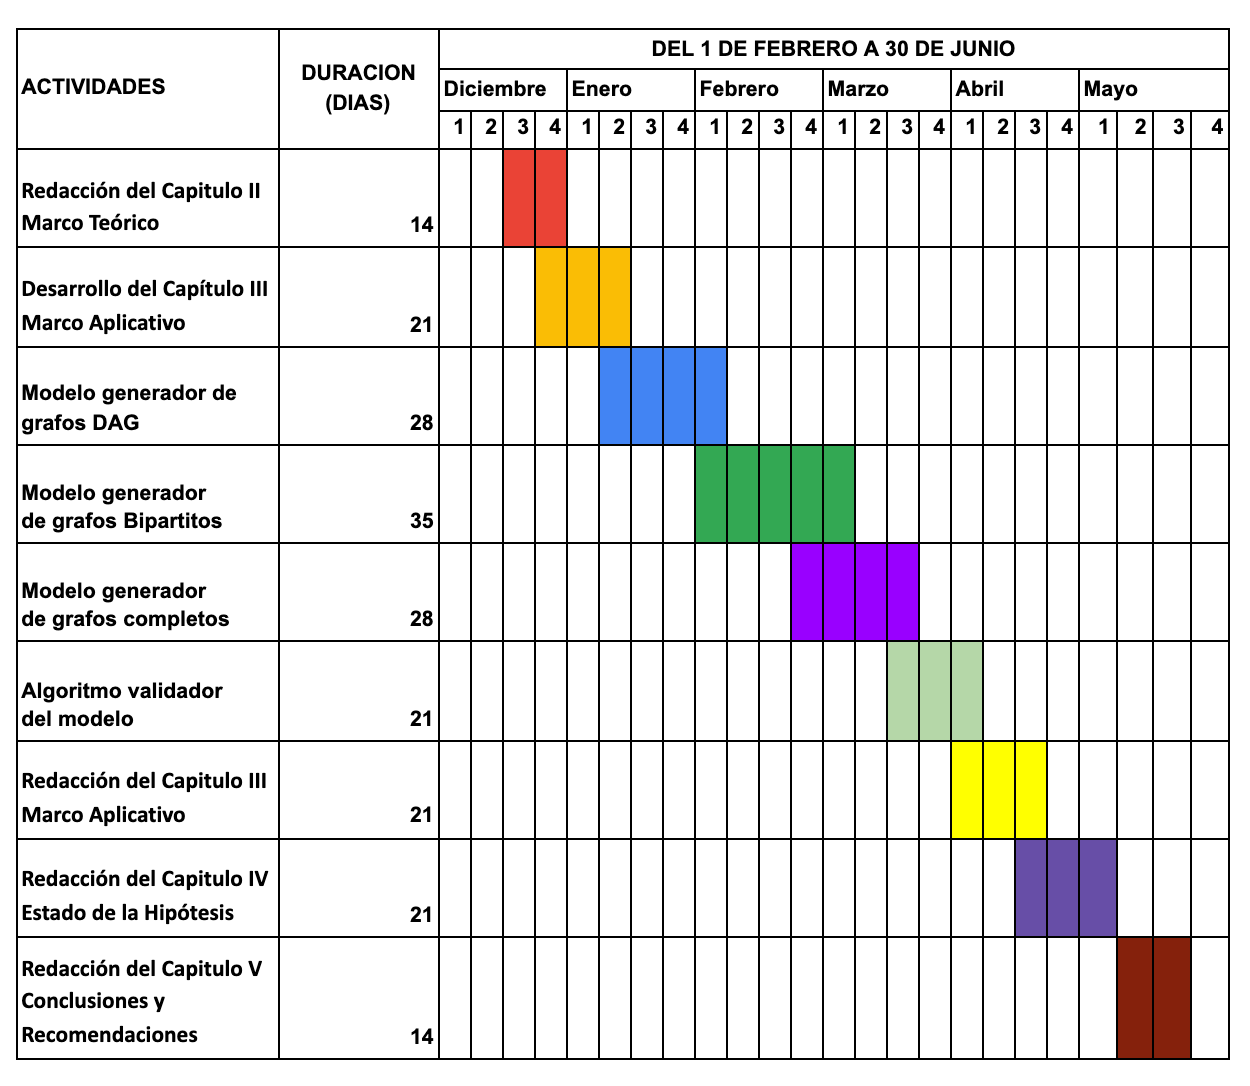
\includegraphics[width=18cm,height=15cm]{calendario.png}
\subsection{Indice de trabajo}
  \begin{enumerate}
    \item CAPÍTULO 1: MARCO REFERENCIAL
    \begin{enumerate}
      \item Introduccion
      \item Antecedentes
      \item Planteamiento del problema
        \begin{enumerate}
          \item Problema central
          \item Problemas secundarios
        \end{enumerate}
      \item Objetivo
        \begin{enumerate}
          \item Objetivo principal
          \item objectivos secundarios
        \end{enumerate}
      \item Hip\'otesis
      \item \justificacion
        \begin{enumerate}
          \item \justificacion econ\'omica
          \item \justificacion social
          \item \justificacion cient\'ifica
        \end{enumerate}
      \item Alcances y L\'imites
        \begin{enumerate}
          \item Alcances
          \item L\'imites
        \end{enumerate}
      \item Metodolog\'ia
    \end{enumerate}
    \item CAPITULO 2: MARCO TEORICO
      \begin{enumerate}
        \item Mascaras de bits
        \begin{enumerate}
          \item Operaciones con mascaras de bits
        \end{enumerate}
        \item Programac\'ion din\'amica (DP)
        \begin{enumerate}
          \item DP con mascaras de bits
        \end{enumerate}
        \item Teor\'ia de grafos
        \begin{enumerate}
          \item Grafos ac\'iclicos no diridos (DAG)
          \item Grafos Bipartitos
          \item Grafos completos
          \item Caminos y ciclos hamiltonianos
        \end{enumerate}
        \item{Grafos aleatorios}
        \begin{enumerate}
          \item Modelo de Erdös-Rényi
          \item Modelo de Configuraciones
          \item Otros modelos de grafos aleatorios
        \end{enumerate}
        \item Cadenas de Markov
      \end{enumerate}
    \item CAPITULO 3: MARCO APLICATIVO
      \begin{enumerate}
        \item Modelo generador de grafos DAG
        \item Modelo generador de grafos Bipartitos 
        \item Modelo generador de grafos completos
        \item Algoritmo validdor del modelo
      \end{enumerate}
    \item CAPITULO 4: AN\'ALISIS Y RESULTADOS
      \begin{enumerate}
        \item Complejidad algoritmica.
        \item Demostracion de la mejora con respecto a otros modelos.
      \end{enumerate}
    \item CAPITULO 5:
      \begin{enumerate}
        \item Conclusiones
        \item Recomendaciones
      \end{enumerate}
    \item Bibliograf\'ia
    \item Anexos
  \end{enumerate}
\end{document}
